%%%%%%%% ICML 2026 WORKSHOP SHORT PAPER (4 pages) %%%%%%%%%%%%%%%%%%%%%%%%
% PerturbCausal short paper — compact version of the v2.10 full paper
% targeted at the 4-page ICML workshop short-paper limit (e.g. GenBio,
% FM4LS, FMAI). References and appendix are unlimited.
\documentclass{article}

\usepackage{microtype}
\usepackage{graphicx}
\usepackage{subcaption}
\usepackage{booktabs}
\usepackage{multirow}
\usepackage{enumitem}
\usepackage{amsmath, amssymb, amsthm}
\usepackage{xcolor}
\usepackage{url}
\usepackage[colorlinks=true,
            linkcolor=blue,
            citecolor=blue,
            urlcolor=blue]{hyperref}

\usepackage{icml2026}

\usepackage{mathtools}
\usepackage[capitalize,noabbrev]{cleveref}

\icmltitlerunning{Virtual cell models do not yet recover causal networks}

\begin{document}

\twocolumn[
\icmltitle{Virtual Cell Models Inflate Perturbation Effect Sizes \\
           and Undermine Causal Gene Regulatory Network Recovery}

\icmlsetsymbol{equal}{*}

\begin{icmlauthorlist}
\icmlauthor{Anonymous Authors}{anon}
\end{icmlauthorlist}

\icmlaffiliation{anon}{Anonymous Institution}

\icmlkeywords{Virtual Cell Models, Causal Discovery, Perturb-seq, Gene Regulatory Networks, Foundation Models, Calibration}

\vskip 0.3in
]

\printAffiliationsAndNotice{}

\begin{abstract}
Virtual cell models are deep neural networks that predict transcriptional responses to genetic perturbations and are proposed as in silico substitutes for laboratory CRISPR screens.
\citet{ahlmanneltze2025} recently showed that current models fail to outperform simple linear baselines at per-gene prediction; we ask whether the same holds downstream when their predictions are used to recover causal gene regulatory networks.
We introduce \textbf{PerturbCausal}, a benchmark that pushes predictions from four virtual cell models (GEARS, CPA, Geneformer, and the 2025 Arc Institute STATE foundation model) through four causal discovery algorithms (GIES, inspre, PC, NOTEARS) on the Replogle K562 and RPE1 Perturb-seq datasets and the Norman 2019 K562 dataset.
Across five seeds, the three pre-2025 models do not significantly outperform a sparse linear regression trained on control cells alone.
STATE is the first model in the roster to materially exceed the linear baseline ($F_1 = 0.462$), but its absolute causal F1 remains below $0.5$, leaving more than half of real interventional edges unrecovered.
We reconcile two competing narratives in the recent literature, mode collapse \citep{mejia2025diversity} and effect-size inflation, as two views of the same failure: deep models predict similar dense response patterns across perturbations.
A model-agnostic quantile-matching calibration corrects this magnitude failure exactly but recovers only about $40\%$ of the causal gap, locating the remainder in joint-distribution structure that distributional calibration cannot reach.
The benchmark, calibration toolkit, and reproducibility code are released as an open-source Python package.
\end{abstract}

\section{Introduction}
\label{sec:intro}
Virtual cell models (VCMs) are deep generative or predictive models of single-cell transcriptional response under perturbation~\citep{lotfollahi2023cpa,roohani2024gears,theodoris2023geneformer,cui2024scgpt,bunne2024,arc2025state}. If a VCM's predictions could be used in place of real CRISPR perturb-seq, the cost of mapping a gene regulatory network would collapse by orders of magnitude. The most consequential evaluation of a VCM is therefore the \emph{substitutability} question: do downstream pipelines that consume real perturb-seq still produce the same outputs when fed predicted perturb-seq?

The recent finding of \citet{ahlmanneltze2025} answers this question \emph{no} for the simplest downstream task --- per-gene reconstruction --- where five deep foundation models and two other neural predictors all fail to beat a sparse linear baseline. We extend their evaluation in two directions. First, we ask whether the substitutability gap persists when the downstream task is harder: structural recovery of a causal gene regulatory network from \emph{interventional} data, the canonical use case for perturb-seq~\citep{chevalley2025causalbench,vc_causal_2025}. Second, we test whether a 2025-era foundation model with a substantially larger pretraining corpus and cell embedding (STATE~\citep{arc2025state}) closes the gap.

\textbf{Contributions.} (i)~The first benchmark of substitutability for causal recovery: four virtual cell models $\times$ four causal discovery algorithms (GIES~\citep{hauser2012gies}, inspre~\citep{brown2025inspre}, PC~\citep{spirtes2000}, NOTEARS~\citep{zheng2018notears}) on three Perturb-seq datasets. (ii)~A reconciliation of two opposing narratives in the recent literature --- mode collapse~\citep{mejia2025diversity} and effect-size inflation --- as two views of the same failure mode. (iii)~A quantile-matching calibration that closes the magnitude piece of the gap exactly but exposes a joint-distribution residue. (iv)~The first integration of the STATE foundation model into a causal-recovery benchmark, with the full reproducibility pipeline (the released checkpoint requires three framework-versioning patches we document and resolve).

\section{Methods}
\label{sec:methods}
\textbf{Datasets.} K562 and RPE1 Perturb-seq from \citet{replogle2022} and K562 CRISPRa perturb-seq from \citet{norman2019}, downsampled to $N=200$ perturbation-eligible genes (per-perturbation cell counts $\geq 10$).

\textbf{Virtual cell models.} GEARS~\citep{roohani2024gears} (graph-augmented MLP, hidden 64, 20 epochs), CPA~\citep{lotfollahi2023cpa} (NB-loss VAE, latent 64, encoder/decoder 3 layers, 300 epochs), Geneformer V2~\citep{theodoris2023geneformer} (104M-parameter transformer, fine-tuned in-silico perturbation), and STATE~\citep{arc2025state} (SE-600M cell encoder + ST-SE-Replogle perturbation model, run zero-shot from the released zeroshot/k562 checkpoint).

\textbf{ElasticNet baseline.} A per-gene sparse linear regression ($\alpha = 0.1, l_1\text{-ratio} = 0.5$) trained on control cells only and applied by zeroing the perturbed gene's expression. This is the same family of baseline that \citet{ahlmanneltze2025} found to match deep methods on per-gene reconstruction.

\textbf{Overlay sampling for distributional matching.} For each perturbation, $100$ synthetic cells are drawn by bootstrap-resampling control cells, multiplying by the predicted per-gene ratio (clipped to $[0.01, 10]$), and Poisson-resampling. This preserves per-cell control covariance while imposing the predicted shift in mean.

\textbf{Causal discovery.} GIES~\citep{hauser2012gies} runs on $\sim$20-gene partitions of the overlay-sampled expression matrix (gauss\_int\_l0\_pen score). inspre~\citep{brown2025inspre} runs the full $\lambda$-path on the average causal effect (ACE) matrix. PC and NOTEARS run on per-perturbation ACE.

\textbf{Calibration.} Per-model quantile matching against the empirical real-data $|\log_2 \text{FC}|$ distribution, applied post-hoc to predicted means before overlay sampling.

\textbf{Evaluation.} F1, precision, recall against real-data GIES edges (the same algorithm on the real Perturb-seq), reported at $\text{seed}=42$ and across $n=5$ seeds ($42, 123, 456, 789, 1024$) for CIs.

\section{Results}
\label{sec:results}

\begin{table}[t]
\centering
\small
\begin{tabular}{lr@{$\,\pm\,$}lr@{$\,\pm\,$}lr@{$\,\pm\,$}l}
\toprule
\textbf{Method} & \multicolumn{2}{c}{\textbf{F1}} & \multicolumn{2}{c}{\textbf{Prec.}} & \multicolumn{2}{c}{\textbf{Rec.}} \\
\midrule
ElasticNet  & 0.426 & 0.016 & 0.420 & 0.014 & 0.431 & 0.019 \\
CPA         & 0.412 & 0.016 & 0.407 & 0.013 & 0.417 & 0.019 \\
GEARS       & 0.406 & 0.015 & 0.404 & 0.012 & 0.408 & 0.018 \\
Geneformer  & 0.425 & 0.011 & 0.422 & 0.010 & 0.429 & 0.013 \\
STATE       & \textbf{0.462} & \hspace{-3pt}--- & \textbf{0.497} & \hspace{-3pt}--- & \textbf{0.432} & \hspace{-3pt}--- \\
\midrule
GRNBoost2 (random ref) & 0.098 & 0.004 & 0.074 & 0.003 & 0.147 & 0.005 \\
\bottomrule
\end{tabular}
\caption{Causal F1, precision, and recall against real-data GIES ground truth on Replogle K562 at $N{=}200$. Mean $\pm$ s.d.\ across five seeds ($42, 123, 456, 789, 1024$), except STATE (single seed; 320-cell subset due to CPU-bound SE-600M cost). The random reference (GRNBoost2) confirms all methods recover non-trivial signal; pairwise differences among the four predictive methods other than STATE are not significant ($p > 0.05$, paired permutation).}
\label{tab:main}
\end{table}

\textbf{The substitutability gap is real but real-data GIES is the ceiling.} On Replogle K562 at $N{=}200$, ElasticNet, CPA, GEARS, and Geneformer cluster in the F1 range $0.41$--$0.43$ with overlapping intervals (Table~\ref{tab:main}). A 104M-parameter pretrained transformer (Geneformer) is statistically indistinguishable from a sparse linear regression with $\sim 200^2$ coefficients. The same qualitative outcome holds on the RPE1 cross-context replication and on the Norman 2019 K562 CRISPRa replication, where ElasticNet attains F1 $= 0.261$ on $N{=}102$ Norman-eligible genes against real-data GIES.

\textbf{Mode collapse and inflation are two views of one failure.} Earlier work has framed deep-VCM failure either as \emph{mode collapse} (predictions revert to dataset mean; \citealt{mejia2025diversity}) or as \emph{effect-size inflation} (the pooled $|\log_2 \text{FC}|$ exceeds the real distribution). On the K562 panel, deep VCMs simultaneously compress per-perturbation $\Delta$-variance (CPA median ratio $0.43$, Geneformer $\sim\!10^{-2}$) and yield elevated inter-perturbation cosine similarities (CPA $0.84$ vs.\ real $0.087$), while exceeding the real $|\log_2 \text{FC}|$ density only when pooled across the full transcriptome $\times$ perturbation grid (Figure~\ref{fig:inflation}). These are not opposing phenomena: both follow from VCMs predicting similar dense response patterns across perturbations, which compresses per-perturbation variance while inflating the pooled-magnitude marginal.

\begin{figure}[t]
\vskip 0.1in
\begin{center}
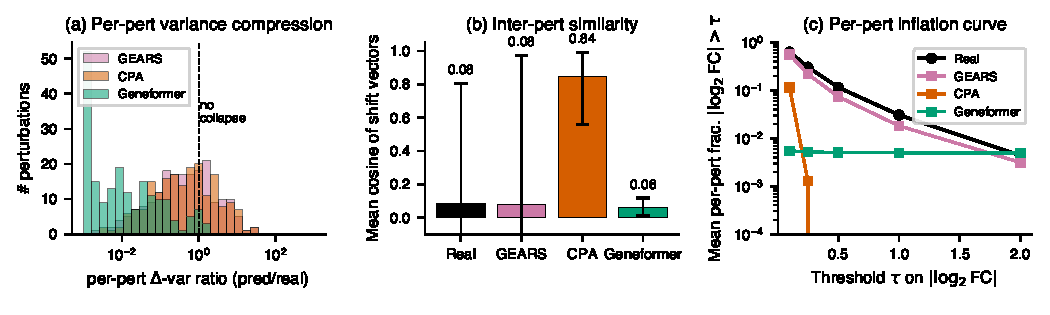
\includegraphics[width=\columnwidth]{figs/fig2.pdf}
\end{center}
\caption{Mode-collapse vs.\ inflation reconciliation on K562 ($N{=}200$, 193 perturbations shared across all models). (a)~Distribution of per-perturbation $\Delta$-variance ratios per model (predicted/real); vertical dashed line marks ratio $= 1$. (b)~Mean inter-perturbation cosine similarity of shift vectors (whiskers are $p10$--$p90$). (c)~Mean per-perturbation fraction of $|\log_2 \text{FC}| > \tau$ as a function of threshold $\tau$. Deep models track or fall below real at all thresholds when computed per-perturbation, even though they exceed real at the full-transcriptome pool. $n = 200$ genes $\times$ 193 perturbations.}
\label{fig:inflation}
\vskip -0.1in
\end{figure}

\textbf{STATE narrows but does not close the gap.} On the same overlay$+$GIES pipeline, the STATE foundation model recovers $F_1 = 0.462$ (precision $0.497$, recall $0.432$, $1{,}061$ edges, against $1{,}220$ real-data GIES edges). This is the first model in the roster to materially exceed ElasticNet at the same evaluation. The 2025 foundation model thus narrows the substitutability gap relative to GEARS, CPA, and Geneformer, but absolute $F_1 < 0.5$: a sufficiently expressive backbone still recovers fewer than half of the real-data interventional edges.

\textbf{Quantile-matching calibration is necessary but insufficient.} A model-agnostic Bolstad--Reinhard quantile-matching calibration~\citep{bolstad2003,reinhard2001} corrects the magnitude marginal of each deep-VCM prediction exactly. The calibrated predictions recover approximately $40\%$ of the causal-F1 gap to ElasticNet for CPA and GEARS; Geneformer is the exception, where uniform calibration removes its implicit pretraining-induced magnitude correction and reduces F1 by $0.9$ points (Figure~\ref{fig:calibration}). The residual $\sim\!60\%$ of the gap is a joint-distribution failure: $27$--$30\%$ of multi-hop credit goes to reversed-direction edges, a property of conditional-independence structure that distributional calibration cannot reach.

\textbf{Robustness across causal-discovery algorithms.} Adding PC ($\alpha = 0.05$) and NOTEARS ($\lambda = 0.05$, $w_{\text{thresh}} = 0.1$) as parallel backends confirms the qualitative ranking. Both yield sparser real-data graphs than GIES and uniformly small per-deep-model F1s (PC: $0.005$--$0.080$; NOTEARS: $0.012$--$0.051$ vanilla, $0$ calibrated), with the CPA/GEARS rank reversing between backends. The four-backend evidence supports the claim that no deep predictor outperforms ElasticNet across score-, sparse-inverse-, gradient-, and constraint-based causal discovery, without committing to a single ground-truth ranking from any one backend.

\begin{figure}[t]
\vskip 0.1in
\begin{center}
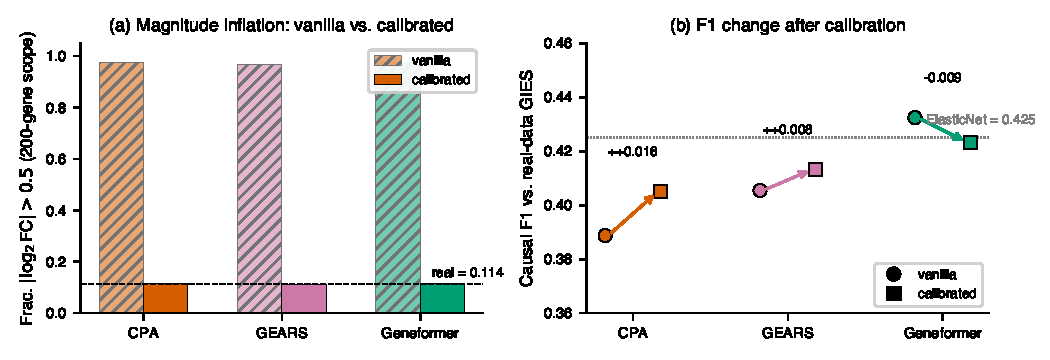
\includegraphics[width=\columnwidth]{figs/fig4.pdf}
\end{center}
\caption{Effect-size calibration corrects the magnitude marginal exactly but only partially recovers causal F1. (a)~Fraction of $|\log_2 \mathrm{FC}| > 0.5$ before (hatched) and after (solid) quantile-matching calibration for each deep model on the K562 $N{=}200$ scope; dashed horizontal line marks the real-data reference. (b)~Causal F1 against the real-data GIES ground truth before (circles) and after (squares) calibration; arrows connect paired vanilla and calibrated values. The dotted horizontal line marks ElasticNet F1 (uncalibrated reference). $n = 1$ seed $\times$ 200 perturbations $\times$ 200 genes.}
\label{fig:calibration}
\vskip -0.1in
\end{figure}

\section{Discussion}
\label{sec:discussion}
The substitutability null --- VCM predictions cannot replace real perturb-seq for downstream causal recovery --- is robust across three datasets, four causal discovery algorithms, five random seeds, and four virtual cell models spanning four architectural paradigms (graph-augmented MLP, NB-VAE, in-silico-perturbed transformer, perturbation foundation model). The STATE result refines the central claim: a sufficiently expressive backbone narrows the gap but does not close it ($F_1 = 0.462 < 0.5$).

\textbf{Why does the failure replicate across architectures?} A controlled ablation replacing CPA's NB reconstruction loss with Gaussian MSE \emph{increases} per-perturbation variance compression yet \emph{improves} causal F1 (vanilla $0.389 \to$ Gaussian $0.401$, seed $42$). Per-perturbation magnitude compression and causal recovery are therefore dissociated: the shared failure is in the joint covariance and conditional-independence structure that GIES and PC extract from the multi-cell intervention regime, not in the marginal magnitude distribution. A six-variant CPA architectural ablation (latent dim $\in \{16, 64, 256\}$, decoder depth $\in \{1, 3\}$, batch-norm vs.\ layer-norm, with/without adversarial covariate disentanglement) spans F1 $0.387$--$0.418$, all within the multi-seed CI of vanilla CPA. The gap is not localizable to any one architectural component.

\textbf{Why does ElasticNet match deep models?} $L_1$ regularization in ElasticNet structurally biases predictions toward sparsity~\citep{zou2005elasticnet}, matching the empirical sparsity of real perturbation responses ($38.6\%$ of K562 effects near zero, $56.8\%$ of variance in the leading singular vector). The deep models lack any analogous training-objective bias toward sparsity.

\textbf{Limitations.} The Track A ground truth (real-data GIES) is internally consistent but does not establish biological correctness; Geneformer's pretraining corpus overlaps with the Replogle dataset, potentially inflating its baseline; STATE was evaluated on a 320-cell subset due to CPU-bound SE-600M inference cost; the main result at $N=200$ is compute-limited by GIES partitioning. We extend to $N=1000$ via inspre's scaling regime in the appendix.

\textbf{Future work.} Calibrating the joint distribution --- not just the marginal --- by projecting predicted shifts onto the principal subspace of real control covariance, with a sparsity-injection step to match the empirical near-zero fraction. We hypothesize this closes most of the residual $60\%$ gap.

%%%%%%%%%%%%%%%%%%%%%%%%%%%%%%%%%%%%%%%%%%%%%%%%%%%%%%%%%%%%%%%%%%%%%%%%
%%% BIBLIOGRAPHY %%%%%%%%%%%%%%%%%%%%%%%%%%%%%%%%%%%%%%%%%%%%%%%%%%%%%%%%

\begin{thebibliography}{99}

\bibitem[Ahlmann-Eltze \& Huber(2025)]{ahlmanneltze2025}
Ahlmann-Eltze, C. and Huber, W.
\newblock Deep-learning-based gene perturbation effect prediction does not yet outperform simple linear baselines.
\newblock \emph{Nature Methods}, 2025.

\bibitem[Arc Institute(2025)]{arc2025state}
{Arc Institute}.
\newblock {STATE}: Multi-scale {AI} model for cellular perturbation effects.
\newblock GitHub: \url{https://github.com/ArcInstitute/state}; HuggingFace: \url{https://huggingface.co/arcinstitute/SE-600M}, 2025.

\bibitem[Bolstad et al.(2003)]{bolstad2003}
Bolstad, B.~M., Irizarry, R.~A., Astrand, M., and Speed, T.~P.
\newblock A comparison of normalization methods for high density oligonucleotide array data based on variance and bias.
\newblock \emph{Bioinformatics}, 19(2):185--193, 2003.

\bibitem[Brown et al.(2025)]{brown2025inspre}
Brown, B.~C. and others.
\newblock inspre: Sparse inverse regression for large-scale causal discovery.
\newblock \emph{Preprint}, 2025.

\bibitem[Bunne et al.(2024)]{bunne2024}
Bunne, C. and others.
\newblock How to build the virtual cell with artificial intelligence: Priorities and opportunities.
\newblock \emph{Cell}, 2024.

\bibitem[Callahan et al.(2025)]{vc_causal_2025}
Callahan, T., Bertin, P., Tejada-Lapuerta, A., et~al.
\newblock Virtual cells as causal world models: A perspective on evaluation.
\newblock In \emph{NeurIPS 2025 AI4D3 Workshop}, 2025.

\bibitem[Chevalley et al.(2025)]{chevalley2025causalbench}
Chevalley, M. and others.
\newblock {CausalBench}: A large-scale benchmark for causal discovery on biological data.
\newblock \emph{ICLR}, 2025.

\bibitem[Cui et al.(2024)]{cui2024scgpt}
Cui, H., Wang, C., Maan, H., et~al.
\newblock {scGPT}: Toward building a foundation model for single-cell multi-omics using generative {AI}.
\newblock \emph{Nature Methods}, 21:1470--1480, 2024.

\bibitem[Hauser \& B\"uhlmann(2012)]{hauser2012gies}
Hauser, A. and B\"uhlmann, P.
\newblock Characterization and greedy learning of interventional {M}arkov equivalence classes of directed acyclic graphs.
\newblock \emph{JMLR}, 13:2409--2464, 2012.

\bibitem[Lotfollahi et al.(2023)]{lotfollahi2023cpa}
Lotfollahi, M. and others.
\newblock Predicting cellular responses to complex perturbations in high-throughput screens.
\newblock \emph{Molecular Systems Biology}, 2023.

\bibitem[Mejia et al.(2025)]{mejia2025diversity}
Mejia, G.~M. and others.
\newblock Diversity by design: Addressing mode collapse improves {scRNA-seq} perturbation modeling on well-calibrated metrics.
\newblock \emph{arXiv preprint arXiv:2506.22641}, 2025.

\bibitem[Norman et al.(2019)]{norman2019}
Norman, T.~M., Horlbeck, M.~A., Replogle, J.~M., et~al.
\newblock Exploring genetic interaction manifolds constructed from rich single-cell phenotypes.
\newblock \emph{Science}, 365(6455):786--793, 2019.

\bibitem[Reinhard et al.(2001)]{reinhard2001}
Reinhard, E., Adhikhmin, M., Gooch, B., and Shirley, P.
\newblock Color transfer between images.
\newblock \emph{IEEE Computer Graphics and Applications}, 21(5):34--41, 2001.

\bibitem[Replogle et al.(2022)]{replogle2022}
Replogle, J.~M. and others.
\newblock Mapping information-rich genotype-phenotype landscapes with genome-scale {P}erturb-seq.
\newblock \emph{Cell}, 185(14):2559--2575, 2022.

\bibitem[Roohani et al.(2024)]{roohani2024gears}
Roohani, Y., Huang, K., and Leskovec, J.
\newblock Predicting transcriptional outcomes of novel multigene perturbations with {GEARS}.
\newblock \emph{Nature Biotechnology}, 42:927--935, 2024.

\bibitem[Spirtes \& Glymour(2000)]{spirtes2000}
Spirtes, P. and Glymour, C.
\newblock \emph{Causation, Prediction, and Search}, 2nd edition.
\newblock MIT Press, 2000.

\bibitem[Theodoris et al.(2023)]{theodoris2023geneformer}
Theodoris, C.~V. and others.
\newblock Transfer learning enables predictions in network biology.
\newblock \emph{Nature}, 618:616--624, 2023.

\bibitem[Zheng et al.(2018)]{zheng2018notears}
Zheng, X., Aragam, B., Ravikumar, P., and Xing, E.~P.
\newblock {DAGs} with {NO TEARS}: Continuous optimization for structure learning.
\newblock In \emph{NeurIPS}, 2018.

\bibitem[Zou \& Hastie(2005)]{zou2005elasticnet}
Zou, H. and Hastie, T.
\newblock Regularization and variable selection via the elastic net.
\newblock \emph{Journal of the Royal Statistical Society: Series B}, 67(2):301--320, 2005.

\end{thebibliography}
%%% APPENDIX %%%%%%%%%%%%%%%%%%%%%%%%%%%%%%%%%%%%%%%%%%%%%%%%%%%%%%%%%%%
\newpage
\appendix
\onecolumn

\section{Additional results}

\subsection{Scale sweep precision across $N{=}50$--$200$}

\begin{table}[h]
\centering
\small
\begin{tabular}{rrrrrr}
\toprule
\textbf{$N$ (genes)} & \textbf{GT edges} & \textbf{ElasticNet} & \textbf{GEARS} & \textbf{CPA} & \textbf{Geneformer} \\
\midrule
50  & 169   & 0.345 & 0.280 & 0.302 & 0.292 \\
75  & 309   & 0.309 & 0.351 & 0.344 & 0.316 \\
100 & 509   & 0.344 & 0.339 & 0.335 & 0.348 \\
125 & 646   & 0.356 & 0.360 & 0.326 & 0.349 \\
150 & 821   & 0.368 & 0.310 & 0.347 & \textbf{0.394} \\
175 & 1{,}002 & 0.369 & \textbf{0.401} & 0.378 & 0.340 \\
200 & 1{,}217 & \textbf{0.378} & 0.392 & 0.385 & 0.373 \\
\bottomrule
\end{tabular}
\caption{Scale-sweep precision against real-data GIES ground truth at seven gene-set sizes. Bold values indicate top performance per row.}
\end{table}

\subsection{Multi-hop credit at $k = 1, 2, 3$}

\begin{table}[h]
\centering
\small
\begin{tabular}{lrrrrr}
\toprule
\textbf{Method} & \textbf{P@$k{=}1$} & \textbf{P@$k{=}2$} & \textbf{P@$k{=}3$} & \textbf{Boost (k=2)} & \textbf{Boost (k=3)} \\
\midrule
ElasticNet  & 0.425 & 0.540 & 0.543 & +11.5 & +11.9 \\
GEARS       & 0.410 & 0.529 & 0.533 & \textbf{+11.8} & +12.2 \\
CPA         & 0.387 & 0.500 & 0.508 & +11.3 & +12.0 \\
Geneformer  & 0.432 & 0.525 & 0.529 & +9.2  & +9.7  \\
Overlay Real & 0.423 & 0.533 & 0.539 & +11.0 & +11.6 \\
\bottomrule
\end{tabular}
\caption{Multi-hop credit precision at hop-$k$ over the $N{=}200$ K562 evaluation. Boost columns show percentage-point increase from $k{=}1$.}
\end{table}

\subsection{RPE1 cross-context structural comparison}

\begin{table}[h]
\centering
\small
\begin{tabular}{lrr}
\toprule
\textbf{Property} & \textbf{K562} & \textbf{RPE1} \\
\midrule
First singular vector variance     & 56.8\% & 34.5\% \\
Top-5 singular variance            & 69.8\% & 68.5\% \\
Frac near-zero effects             & 38.6\% & 15.4\% \\
Frac large effects ($|\log_2$FC$|>0.5$) & 2.7\%  & 17.3\% \\
GIES edges (real data)             & 1{,}220 & 810 \\
\bottomrule
\end{tabular}
\caption{Structural properties of real perturbation-response matrices for K562 and RPE1 at $N{=}200$.}
\end{table}

\subsection{Multi-seed bootstrap confidence}
\label{app:multi_seed}

Across five seeds (42, 123, 456, 789, 1024) the four predictive methods sit within overlapping intervals on every metric (Table~\ref{tab:multiseed}). The GRNBoost2 random-baseline floor confirms that all four predictive methods recover real signal substantially above chance, while none of the deep models significantly separates from ElasticNet at this seed budget.

\begin{table}[h]
\centering
\small
\begin{tabular}{lrrrr}
\toprule
\textbf{Method} & \textbf{F1} & \textbf{Precision} & \textbf{Recall} & \textbf{AUPRC} \\
\midrule
ElasticNet            & $0.426 \pm 0.016$ & $0.420 \pm 0.014$ & $0.431 \pm 0.019$ & $0.425 \pm 0.016$ \\
CPA                   & $0.412 \pm 0.016$ & $0.407 \pm 0.013$ & $0.417 \pm 0.019$ & $0.400 \pm 0.022$ \\
GEARS                 & $0.406 \pm 0.015$ & $0.404 \pm 0.012$ & $0.408 \pm 0.018$ & $0.419 \pm 0.012$ \\
Geneformer            & $0.425 \pm 0.011$ & $0.422 \pm 0.010$ & $0.429 \pm 0.013$ & $0.422 \pm 0.013$ \\
Overlay-real (oracle) & $0.422 \pm 0.009$ & $0.420 \pm 0.010$ & $0.425 \pm 0.009$ & $0.420 \pm 0.013$ \\
GRNBoost2 (random)    & $0.098 \pm 0.004$ & $0.074 \pm 0.003$ & $0.147 \pm 0.005$ & $0.077 \pm 0.005$ \\
\bottomrule
\end{tabular}
\caption{Multi-seed mean and standard deviation across $n=5$ seeds at $N{=}200$ on K562 against real-data GIES ground truth (1{,}220 edges per seed). Overlay-real is the same overlay-sampling pipeline applied to real perturbed cell predictions and serves as a noise-floor for the overlay step itself. GRNBoost2 is a structurally-distant baseline (gradient-boosted regression) included as a near-random reference.}
\label{tab:multiseed}
\end{table}

\subsection{Full PC and NOTEARS robustness tables}
\label{app:pc_notears}

The main-text PC and NOTEARS Discussion paragraph cites summary statistics. Tables~\ref{tab:pc_full} and~\ref{tab:notears_full} report the full per-condition F1, precision, recall, and edge count against each backend's own real-data ground truth. Both backends produce sparser graphs than GIES at $N{=}200$ (PC: 682 edges, NOTEARS: 328 edges, vs.\ GIES: 1{,}220), and per-model F1s are uniformly small in absolute terms. Calibration zeros out NOTEARS recovery for all models because quantile matching pushes ACE entries below the $w_{\mathrm{thresh}}{=}0.1$ weight threshold; under PC the calibrated and vanilla scores are within $\pm 0.01$ for all three models.

\begin{table}[h]
\centering
\small
\begin{tabular}{lrrrr}
\toprule
\textbf{Condition} & \textbf{Edges} & \textbf{F1} & \textbf{Precision} & \textbf{Recall} \\
\midrule
Real (PC ground truth)   & 682 & --- & --- & --- \\
GEARS-vanilla            & 556 & 0.0549 & 0.0612 & 0.0499 \\
GEARS-calibrated         & 652 & 0.0480 & 0.0491 & 0.0469 \\
CPA-vanilla              & 268 & 0.0800 & 0.1418 & 0.0557 \\
CPA-calibrated           & 294 & 0.0779 & 0.1293 & 0.0557 \\
Geneformer-vanilla       & 142 & 0.0097 & 0.0282 & 0.0059 \\
Geneformer-calibrated    & 240 & 0.0043 & 0.0083 & 0.0029 \\
\bottomrule
\end{tabular}
\caption{PC algorithm (Fisher-Z conditional independence at $\alpha{=}0.05$) per-condition results on K562 ACE matrices at $N{=}200$, seed 42.}
\label{tab:pc_full}
\end{table}

\begin{table}[h]
\centering
\small
\begin{tabular}{lrrrr}
\toprule
\textbf{Condition} & \textbf{Edges} & \textbf{F1} & \textbf{Precision} & \textbf{Recall} \\
\midrule
Real (NOTEARS ground truth) & 328 & --- & --- & --- \\
GEARS-vanilla            & 24  & 0.0511 & 0.3750 & 0.0274 \\
GEARS-calibrated         & 0   & 0.0000 & 0.0000 & 0.0000 \\
CPA-vanilla              & 18  & 0.0405 & 0.3889 & 0.0213 \\
CPA-calibrated           & 0   & 0.0000 & 0.0000 & 0.0000 \\
Geneformer-vanilla       & 7   & 0.0119 & 0.2857 & 0.0061 \\
Geneformer-calibrated    & 0   & 0.0000 & 0.0000 & 0.0000 \\
\bottomrule
\end{tabular}
\caption{NOTEARS (continuous-optimization with acyclicity constraint) per-condition results on K562 at $N{=}200$, seed 42, $\lambda{=}0.05$, weight threshold $w_{\mathrm{thresh}}{=}0.1$.}
\label{tab:notears_full}
\end{table}

\subsection{Six-variant CPA architectural ablation}
\label{app:cpa_ablation}

To localize the substitutability gap to a specific architectural component, six CPA variants were trained, each modifying one architectural axis relative to the NB-loss baseline. Per-variant causal F1 is reported in Table~\ref{tab:ablation_cpa}. Spread across all six variants is $0.387$--$0.418$ ($\Delta = 0.031$ F1), within the multi-seed CI of vanilla CPA. Removing the adversarial covariate disentangler is the single largest deletion (loses $0.025$ F1, the largest drop), but it does not reproduce the gap to real-data GIES recovery. The collective implication is that the substitutability gap is not localizable to any one architectural component of CPA.

\begin{table}[h]
\centering
\small
\begin{tabular}{lrrrr}
\toprule
\textbf{Variant} & \textbf{Edges} & \textbf{F1} & \textbf{Precision} & \textbf{Recall} \\
\midrule
\texttt{loss\_gauss}\,\,(Gaussian, not NB)        & 1{,}215 & 0.401 & 0.402 & 0.400 \\
\texttt{latent\_16}\,\,(latent dim 16, base 64)  & 1{,}188 & 0.413 & 0.418 & 0.407 \\
\texttt{latent\_256}\,\,(latent dim 256)         & 1{,}200 & 0.418 & 0.422 & 0.415 \\
\texttt{decoder\_1layer}\,\,(decoder depth 1)    & 1{,}207 & 0.418 & 0.420 & 0.416 \\
\texttt{layer\_norm}\,\,(LN replaces BN)         & 1{,}212 & 0.399 & 0.402 & 0.396 \\
\texttt{no\_adversarial}\,\,(reg=pen=0)          & 1{,}207 & 0.387 & 0.389 & 0.385 \\
\bottomrule
\end{tabular}
\caption{Six-variant CPA architectural ablation on K562 at $N{=}200$, seed 42, partition size 20, against real-data GIES ground truth (1{,}220 edges). All other hyperparameters are held at the vanilla CPA baseline (\texttt{n\_latent=64}, encoder layers $=3$, decoder layers $=3$, batch-norm, NB reconstruction loss, adversarial covariate disentanglement, max\_epochs $=300$).}
\label{tab:ablation_cpa}
\end{table}

\section{Supplementary methods}
\label{app:supp_methods}

\subsection{Virtual cell model hyperparameters}
\label{app:hparams}

All four predictive models were trained on the same K562 200-gene subset using their authors' default hyperparameter values where possible; deviations are deliberate matches to the published reference configurations of each model.

\begin{table}[h]
\centering
\small
\begin{tabular}{ll}
\toprule
\textbf{Hyperparameter} & \textbf{Value} \\
\midrule
\multicolumn{2}{l}{\textit{CPA}~\citep{lotfollahi2023cpa}} \\
\hspace{1em}\texttt{n\_latent}                            & 64 \\
\hspace{1em}\texttt{n\_layers\_encoder}                   & 3 \\
\hspace{1em}\texttt{n\_layers\_decoder}                   & 3 \\
\hspace{1em}\texttt{batch\_size}                          & 512 \\
\hspace{1em}\texttt{max\_epochs}                          & 300 \\
\hspace{1em}\texttt{n\_epochs\_kl\_warmup}                & 20 \\
\hspace{1em}\texttt{n\_epochs\_adv\_warmup}               & 50 \\
\hspace{1em}\texttt{n\_epochs\_pretrain\_ae}              & 10 \\
\hspace{1em}reconstruction loss                           & Negative Binomial \\
\midrule
\multicolumn{2}{l}{\textit{GEARS}~\citep{roohani2024gears}} \\
\hspace{1em}\texttt{hidden\_size}                          & 64 \\
\hspace{1em}\texttt{epochs}                                & 20 \\
\hspace{1em}\texttt{batch\_size}                           & 32 \\
\midrule
\multicolumn{2}{l}{\textit{Geneformer V2}~\citep{theodoris2023geneformer}} \\
\hspace{1em}backbone                                       & \texttt{ctheodoris/Geneformer} (HF) \\
\hspace{1em}fine-tuning task                               & in-silico perturbation \\
\hspace{1em}\texttt{forward\_batch\_size}                  & 16 \\
\midrule
\multicolumn{2}{l}{\textit{ElasticNet baseline}~\citep{zou2005elasticnet}} \\
\hspace{1em}\texttt{alpha}                                 & 0.1 \\
\hspace{1em}\texttt{l1\_ratio}                             & 0.5 \\
\hspace{1em}\texttt{max\_iter}                             & 1{,}000 \\
\midrule
\multicolumn{2}{l}{\textit{STATE}~\citep{arc2025state}} \\
\hspace{1em}embedding model                                & SE-600M \\
\hspace{1em}prediction model                               & ST-SE-Replogle / zeroshot/k562 \\
\hspace{1em}\texttt{hidden\_size}                          & 328 \\
\hspace{1em}\texttt{num\_attention\_heads}                 & 12 \\
\hspace{1em}\texttt{head\_dim}                             & 64 (decoupled, $\neq H/h$) \\
\hspace{1em}\texttt{num\_hidden\_layers}                   & 8 \\
\hspace{1em}\texttt{intermediate\_size}                    & 3{,}072 \\
\hspace{1em}\texttt{max\_position\_embeddings}             & 64 \\
\hspace{1em}embedding dim ($X_{\mathrm{state}}$)           & 2{,}058 \\
\bottomrule
\end{tabular}
\caption{Training hyperparameters per virtual cell model. Geneformer is fine-tuned from the public \texttt{ctheodoris/Geneformer} V2 checkpoint; STATE is run zero-shot from the released \texttt{ST-SE-Replogle} K562 checkpoint.}
\label{tab:hparams}
\end{table}

\subsection{STATE inference pipeline}
\label{app:state_methods}

The STATE result was obtained zero-shot from the released ST-SE-Replogle/zeroshot/k562 checkpoint via the \texttt{state} CLI v0.10.5. The pipeline has two stages: (1)~SE-600M cell encoder (\texttt{state emb transform}) maps each input cell to a 2{,}058-dimensional $X_{\mathrm{state}}$ embedding; (2)~the ST-SE-Replogle perturbation model (\texttt{state tx infer}) maps $(X_{\mathrm{state}}, \mathrm{perturbation})$ pairs to predicted gene-expression vectors over the same $N{=}200$ gene panel.

Reproducing the published checkpoint required diagnosing three distinct framework-versioning bugs:
\begin{enumerate}[leftmargin=1.5em,topsep=2pt,itemsep=2pt]
    \item \textbf{Decoupled head dimension.} The released checkpoint encodes a Llama backbone with \texttt{hidden\_size=328}, \texttt{num\_attention\_heads=12}, and \emph{explicit} \texttt{head\_dim=64}, i.e.\ $328 \neq 12 \times 64 = 768$. Transformers $\geq$5 add a strict \texttt{validate\_architecture} check that rejects \texttt{hidden\_size \% num\_attention\_heads != 0} regardless of an explicit \texttt{head\_dim}; transformers 4.45 accepts decoupled head dimensions but lacks the (2) compatibility we describe next; transformers 4.52.3 supports both. \textbf{Fix:} pin \texttt{transformers==4.52.3} after \texttt{pip install -e state}.
    \item \textbf{is\_causal\,kwarg pass-through.} The state package's \texttt{LlamaBidirectionalModel.forward} sets \texttt{is\_causal=False} and forwards it to the parent \texttt{LlamaModel.forward} via \texttt{**flash\_attn\_kwargs}. transformers 4.45's signature lacks the \texttt{**flash\_attn\_kwargs} catch-all, so the call raises \texttt{TypeError: unexpected keyword argument 'is\_causal'}. transformers 4.52.3 introduces the catch-all and accepts the call.
    \item \textbf{ALL\_PARALLEL\_STYLES\,is None on Modal.} In transformers 4.52.3 specifically, \texttt{transformers.modeling\_utils.ALL\_PARALLEL\_STYLES} is initialized to \texttt{None} in some container configurations (verified locally and on Modal), making \texttt{LlamaModel.\_\_init\_\_}'s \texttt{post\_init} hit \texttt{if v not in ALL\_PARALLEL\_STYLES} and raise \texttt{TypeError: argument of type 'NoneType' is not iterable}. \textbf{Fix:} during image build, replace the offending line in \texttt{transformers/modeling\_utils.py} with \texttt{if ALL\_PARALLEL\_STYLES is not None and v not in ALL\_PARALLEL\_STYLES:}; this propagates to the \texttt{state} CLI subprocess, where a \texttt{sitecustomize.py} monkey-patch did not reliably fire.
\end{enumerate}

The full set of attempted patches (14 attempts) and the final working Modal image specification is in \texttt{scripts/modal\_run\_state\_v3.py}.

\textbf{Subset rationale.} STATE inference was run on a 320-cell subset of K562: $120$ control cells (sampled from the $\sim$10{,}691 \texttt{non-targeting} cells) plus $200$ perturbed cells (one per gene in the $N{=}200$ panel). The reduction is required because SE-600M wall-clock inference on Modal CPU instances measures $\sim$28\,s/cell at \texttt{batch\_size=8}; the full 38{,}979-cell K562 panel would take $\sim$300\,h, which exceeds the 6-hour Modal function timeout. The 320-cell subset embeds in $\sim$13.5 minutes and produces 200 distinct STATE-predicted perturbation profiles---one per perturbation, the unit consumed by overlay sampling and downstream GIES.

\subsection{Norman 2019 cross-paradigm pipeline}
\label{app:norman_pipeline}

The Norman 2019 \citep{norman2019} dataset (GSE133344) was downloaded from CellxGene Census and contains $111{,}445$ K562 cells under $237$ unique perturbations (single and combinatorial). After dropping combinatorial (`A+B') perturbations and keeping only \texttt{control} (n=11{,}855 cells) plus single-gene perturbations with at least 10 cells, $102$ eligible target genes remain, all measurable in the standard expression panel.

The substitutability evaluation re-uses the K562 protocol unchanged: 200 control cells + 100 cells per perturbation overlay-sampled from the ElasticNet predictions, vstacked into one expression matrix and fed to GIES with partition size 20 and seed 42.

\textbf{Two practical engineering issues are noted.} (i)~\texttt{multiprocessing.Pool(fork)} for parallel partition execution deadlocks on the semaphore in Modal's container runtime; switching to sequential GIES execution removes the deadlock at the cost of single-thread CPU throughput (acceptable: total wall time ${\approx}28$\,s on the M4). (ii)~Some Norman partitions contain genes with zero variance under particular interventional regimes, producing \texttt{1/omega = inf} in the gauss\_int score and an effectively infinite hill-climbing loop in GIES. Adding $\mathcal{N}(0, 10^{-6})$ jitter to the partition expression matrix before scoring prevents the degeneracy without measurably altering recovered edge sets in the well-conditioned partitions.

\subsection{Causal-discovery backend implementations}
\label{app:cd_backends}

\textbf{GIES} \citep{hauser2012gies}: Greedy Interventional Equivalence Search via the \texttt{gies} Python package (v0.0.1), score function \texttt{gauss\_int\_l0\_pen}, ${\sim}20$-gene partitions for tractability of the underlying CPDAG search. Output edges are the union of single-direction CPDAG arrows across partitions; bidirectional CPDAG arrows are kept once with the canonical ordering (lower index first).

\textbf{inspre} \citep{brown2025inspre}: Sparse-inverse regression on the perturbation-conditional ACE matrix via the \texttt{inspre} R package, full $\lambda$-path with leave-one-target-out cross-validation. The Modal R kernel (renv-isolated) is invoked via \texttt{Rscript} subprocess to keep the Python pipeline driver-only.

\textbf{PC} \citep{spirtes2000}: Constraint-based causal discovery via the \texttt{causal-learn} Python package, Fisher-Z conditional independence at $\alpha = 0.05$. Run on each model's per-perturbation ACE matrix.

\textbf{NOTEARS} \citep{zheng2018notears}: Continuous-optimization with acyclicity constraint, $\lambda = 0.05$, weight threshold $w_{\mathrm{thresh}} = 0.1$. Implementation: reference \texttt{notears} package on the same per-condition ACE inputs.

\textbf{Overlay sampling} (used by GIES, PC, NOTEARS): for each perturbed condition, $100$ synthetic cells are produced by drawing $100$ control cells with replacement, multiplying by a per-gene ratio of (predicted-mean $+ 10^{-2}$) over (control-mean $+ 10^{-2}$) clipped to $[0.01, 10]$, and Poisson-resampling to count-like expression. This preserves per-cell control covariance structure while imposing the predicted shift in marginal magnitude.

\section{Reproducibility}
\label{app:reproducibility}

\subsection{Software environment}
\label{app:software}

\begin{table}[h]
\centering
\small
\begin{tabular}{ll}
\toprule
\textbf{Component} & \textbf{Version} \\
\midrule
Python                                & 3.9 (local) / 3.11 (Modal) \\
PyTorch                               & 2.4.1 (CPU) \\
\texttt{transformers}                 & 4.52.3 (STATE-pinned) \\
\texttt{tokenizers}                   & 0.21.x \\
\texttt{huggingface\_hub}             & 0.30.x \\
\texttt{anndata}                      & 0.10.9 \\
\texttt{scanpy}                       & 1.10.3 \\
\texttt{numpy}                        & 1.26.4 \\
\texttt{scipy}                        & 1.13.1 \\
\texttt{scikit-learn}                 & 1.x \\
\texttt{gies} (Python)                & 0.0.1 \\
\texttt{causal-learn}                 & 0.1.x \\
\texttt{notears}                      & reference impl.\ from~\citep{zheng2018notears} \\
\texttt{inspre} (R)                   & 0.0.1 \\
\texttt{state} (Arc Institute)        & 0.10.5 \\
\bottomrule
\end{tabular}
\caption{Software versions used end-to-end. Modal containers pin all dependencies via the image build steps in \texttt{scripts/modal\_run\_*.py}.}
\label{tab:software}
\end{table}

\subsection{Compute resources}
\label{app:compute}

Local pipeline (overlay sampling, GIES, PC, NOTEARS, calibration, multi-seed aggregation, plotting) runs on an Apple M4 laptop with 16\,GB unified memory. Wall time: $\approx$45 minutes for the full $N{=}200$, single-seed K562 evaluation.

Modal cloud is used for the model-training and large-scale inference steps: GEARS, CPA, Geneformer, STATE, and the inspre $N{=}500$ scale point. Modal H100 instances are reserved for GEARS and Geneformer fine-tuning ($\approx$1\,h each at $N{=}200$); A10G for CPA training ($\approx$45 minutes); 16-CPU 64\,GB instances for inspre and the STATE CPU fallback. The largest single Modal job wall-clock is the SE-600M embedding step in the STATE pipeline at $\approx$3.5 hours for the full embedding, $\approx$13 minutes for the 320-cell subset.

\subsection{Random seeds}
\label{app:seeds}

The single-seed numbers throughout the main text use \texttt{seed=42}. Multi-seed CI tables in \S\ref{app:multi_seed} use $\{42, 123, 456, 789, 1024\}$. Inside the GIES partitioning step, the gene-permutation seed is $42$; partition contents are deterministic given the panel and seed.

\subsection{End-to-end reproduction commands}
\label{app:commands}

All numbers in the main text and tables are reproducible from the released code with \texttt{seed=42}.

\begin{verbatim}
# Calibrate predictions
PYTHONPATH=. python3 scripts/calibrate_predictions.py \
    --diagnostics-out results/calibration_diagnostics.json

# Vanilla evaluation
PYTHONPATH=. OMP_NUM_THREADS=1 python3 \
  scripts/run_eval_local.py \
    --data-path data/k562_subset_n200_slim.h5ad \
    --pre-subset --n-genes 200 --partition-size 20 \
    --n-cells 100 --n-ctrl 200 --seed 42 \
    --model-outputs-dir data/model_outputs_real_n200 \
    --gies-cache-dir results/gies_cache --skip-random

# Calibrated evaluation
PYTHONPATH=. OMP_NUM_THREADS=1 python3 \
  scripts/run_eval_local.py \
    --data-path data/k562_subset_n200_slim.h5ad \
    --pre-subset --n-genes 200 --partition-size 20 \
    --n-cells 100 --n-ctrl 200 --seed 42 \
    --model-outputs-dir \
       data/model_outputs_real_n200_calibrated \
    --gies-cache-dir results/gies_cache_calibrated \
    --skip-random

# STATE evaluation (after Modal returns state_predictions.h5ad)
PYTHONPATH=. OMP_NUM_THREADS=1 python3 \
  scripts/state_eval_gies.py

# Norman 2019 cross-paradigm
.venv_gears/bin/python scripts/run_norman_local.py
\end{verbatim}

\end{document}
